%This is the introduction...
%
%\vspace{0.5cm}
%
%\begin{figure}[]
%  \centering
%  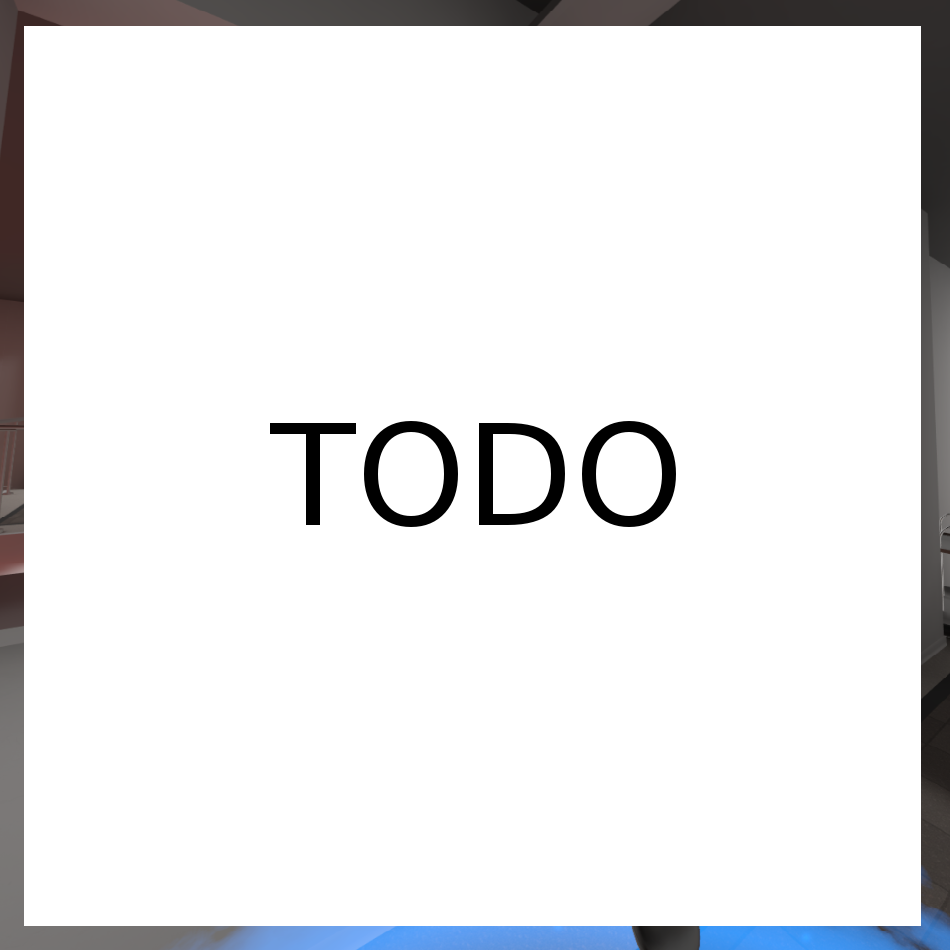
\includegraphics[width=0.5\textwidth]{images/todo.png}
%  \caption{This is an example ToDo picture.}
%  \label{fig:todo}
%\end{figure}
%
%Hypotheses and sub-hypotheses can be formulated like this:
%
%\begin{hypothesis}
%\label{hyp:test}
%This is a hypothesis.
%\end{hypothesis}
%
%\begin{shypothesis}
%\label{shyp:test}
%This is a sub-hypothesis.
%\end{shypothesis}
%
%Hypothesis \cref{hyp:test} is very importance and must be referenced in the text.

Many navigation techniques exist for both Desktop and Immersive \acrfull{ve} that define how users moves around these \acrshort{ve}s. They can be active such that the user is controlling their own movement; passive such that the user is being automatically moved around the environment; or they can be a mix of active and passive. Navigation techniques also have to ensure that there is minimal motion sickness, sufficient environmental awareness which means that while navigating the user knows where they are in an environment compared to where they were before and that it is easy to reach important places in the environment. Two main categories of navigation techniques are Steering and Teleportation.

Steering navigation is 